\section{Architettura di sistema} \label{sec:arch}
L'architettura adottata nella realizzazione dell'applicativo segue le linee guida date dalla Clean Architecture. Il software è stato suddiviso in livelli, in base alla tipologia di logica ad esso riferita, secondo una struttura concentrica.\\
Ogni livello o strato dell'applicativo è indipendente da quelli ad esso più esterni, ovvero nulla presente in un livello più interno può conoscere l'implementazione del livello più esterno.\\
Questo principio alla base dell'architettura clean ci permette di ottenere un prodotto software la cui logica di business è del tutto indipendente dal framework utilizzato per la realizzazione dell'interfaccia grafica e dalle basi di dati adottate.\\
Gli elementi che costituiscono l'architettura sono i seguenti:
\begin{description}
    \item[Controller:] è il punto di ingresso per le richieste dall'esterno del sistema. Esso accetta le richieste in arrivo dall'esterno, utilizza gli use case per effettuare le operazioni richieste e gestisce la conversione dei dati ricevuti nei formati appropriati.
    \item[Use case:] rappresentano le singole funzionalità o casi di utilizzo dell'applicazione. Essi contengono la logica di business. Essi coordinano l'esecuzione delle operazioni richieste dalla logica di business, andando a definire ed implementare le regole di business specifiche di ogni funzionalità. Utilizzano i repository per accedere e manipolare i dati.
    \item[Repository:] sono responsabili per l'accesso ai dati persistenti, fornendo un'interfaccia astratta per la comunicazione con il livello di persistenza dei dati sottostante. Astraggono il resto dell'applicazione dai dettagli tecnici specifici del sistema di persistenza dei dati, fornendo i metodi per recuperare, salvare, aggiornare ed eliminare dati.
    \item[Data source:] sono gli elementi che effettivamente accedono e manipolano i dati nel sistema di persistenza sottostante, forniscono l'implementazione concreta dei metodi per l'accesso ai dati presenti nei repository.
\end{description}
L'adozione di una Clean Architecture come architettura di sistema porta numerosi vantaggi:
\begin{itemize}
    \item Elevato grado di modularità del codice, suddividendolo in base alla logica e alle responsabilità che implementa.
    \item Indipendenza della business logic da qualsiasi framework, tecnologie e interfaccia utente adottata. Ogni cambiamento apportato non compromette il corretto funzionamento del sistema.
    \item Il funzionamento del sistema è completamente indipendente dalle tecnologie utilizzate per i database, con le fonti dei dati che possono essere molteplici. Ogni cambiamento apportato non compromette il corretto funzionamento del sistema.
    \item La leggibilità, la comprensibilità e la testabilità dell'intero sistema è semplificata.
\end{itemize}

\begin{figure}[h!]
    \centering  
    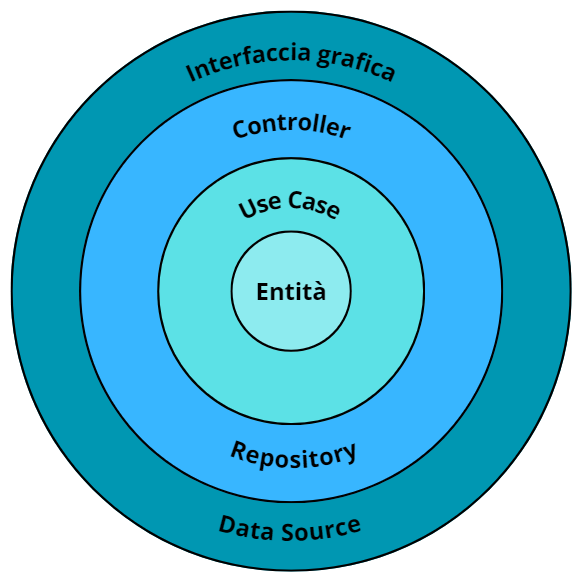
\includegraphics[width=0.5\textwidth]{cleanarch.png}
    \caption{Schema della Clean Architecture}
\end{figure}

\newpage